The first dataset is generated by sequentially generating $\diffx$ and $\diffy$.
First, the $\diffxt$ are sampled as a sum of a standard normal random number and a uniform random number on $(-10, 10)$:
\begin{equation*}
    \diffxt \sim N(0, 1) + U(-10, 10) \quad t = 1, \dots, T.
\end{equation*}
Subsequently, the $\diffy$ are simulated for a constant trending ratio $k$ by
\begin{equation*}
    \diffyt = \diffxt \cdot n_t * b_t,
\end{equation*}
where $n_t$ is a truncated normal distribution with mean 1 and standard deviation 0.5, truncated at 0 and a symmetric Bernoulli random variable with parameter $k$.
For a time-varying trending ratio, the parameter $k$ is modified to have a wave-shape over time, that is,
\begin{equation*}
    k_t = 0.75 + \sin(t / 365.25 \cdot 2 \pi) / 4,
\end{equation*}
where $T^\star$ is $T$ divided by the number of oscillations; in this case, 4.
For the asymmetric trending ratio, $k$ is a function of $\diffxt$,
\begin{equation*}
    k(x) = 0.5 + \min \left\{ \max \left\{ \frac{x + 5}{10}, 0  \right\} , 1 \right\} / 2.
\end{equation*}

In the second approach, $\diffyt$ and $\diffxt$ are modelled to be multivariate normal with mean 0 and covariance matrix
\begin{equation*}
    \Sigma = \begin{pmatrix} 4 & 3 \\ 3 & 4 \end{pmatrix}.
\end{equation*}
Thus, the conditional probability of trending can be calculated by a conditional normal distribution to
\begin{equation*}
    P(\diffyrv \diffxrv > 0 | \diffxrv = x) = \Phi \left( \frac{3}{4 \sqrt{7}} x \right),
\end{equation*}
where $\Phi$ is a standard normal \ac{cdf}.

\begin{figure}
    \centering
    \begin{subfigure}{0.24\textwidth}
        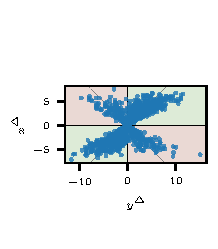
\includegraphics{plots/illustrative_examples/appendix_4q_dgp1}
        \caption{Constant trending ratio.}
    \end{subfigure}\hspace{0.01\textwidth}
    \begin{subfigure}{0.24\textwidth}
        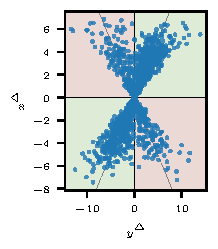
\includegraphics{plots/illustrative_examples/appendix_4q_dgp1_time}
        \caption{Time-varying trending ratio}
    \end{subfigure}\hspace{0.01\textwidth}
    \begin{subfigure}{0.24\textwidth}
        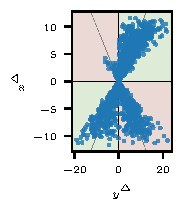
\includegraphics{plots/illustrative_examples/appendix_4q_dgp1_asym}
        \caption{Asymmetric trending ratio}
    \end{subfigure}\hspace{0.01\textwidth}
    \begin{subfigure}{0.24\textwidth}
        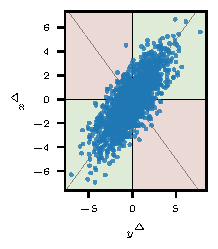
\includegraphics{plots/illustrative_examples/appendix_4q_dgp2}
        \caption{Second approach}
    \end{subfigure}
    \caption{Four-quadrant plots for sample realizations of the data generation schemes of Section~\ref{sec:app-trending-data-generation}. Although the first and second plot differ over time, their difference is not discernible in the plots. The third data set's asymmetry is visible in the plot but the decrese of trending ability near 0 is not visible. }
    \label{fig:appendix_dgps}
\end{figure}
